%% Document the final system design, implementation, and operation.
\chapter{Implemented prototype}
\label{sec:prototype}

%% Show the system components, connections, interfaces, and data flow.
\section{System architecture}

Describe the implemented hardware and software architecture, interfaces,
power paths, and data flow. Include component names and versions where
relevant, and explain how the sensors, PSOC, user interface, and feedback
elements connect. Include a wiring diagram or electrical schematic showing
the relevant connections, pin assignments, and supply voltages.

\begin{figure}[htbp]
  \centering
  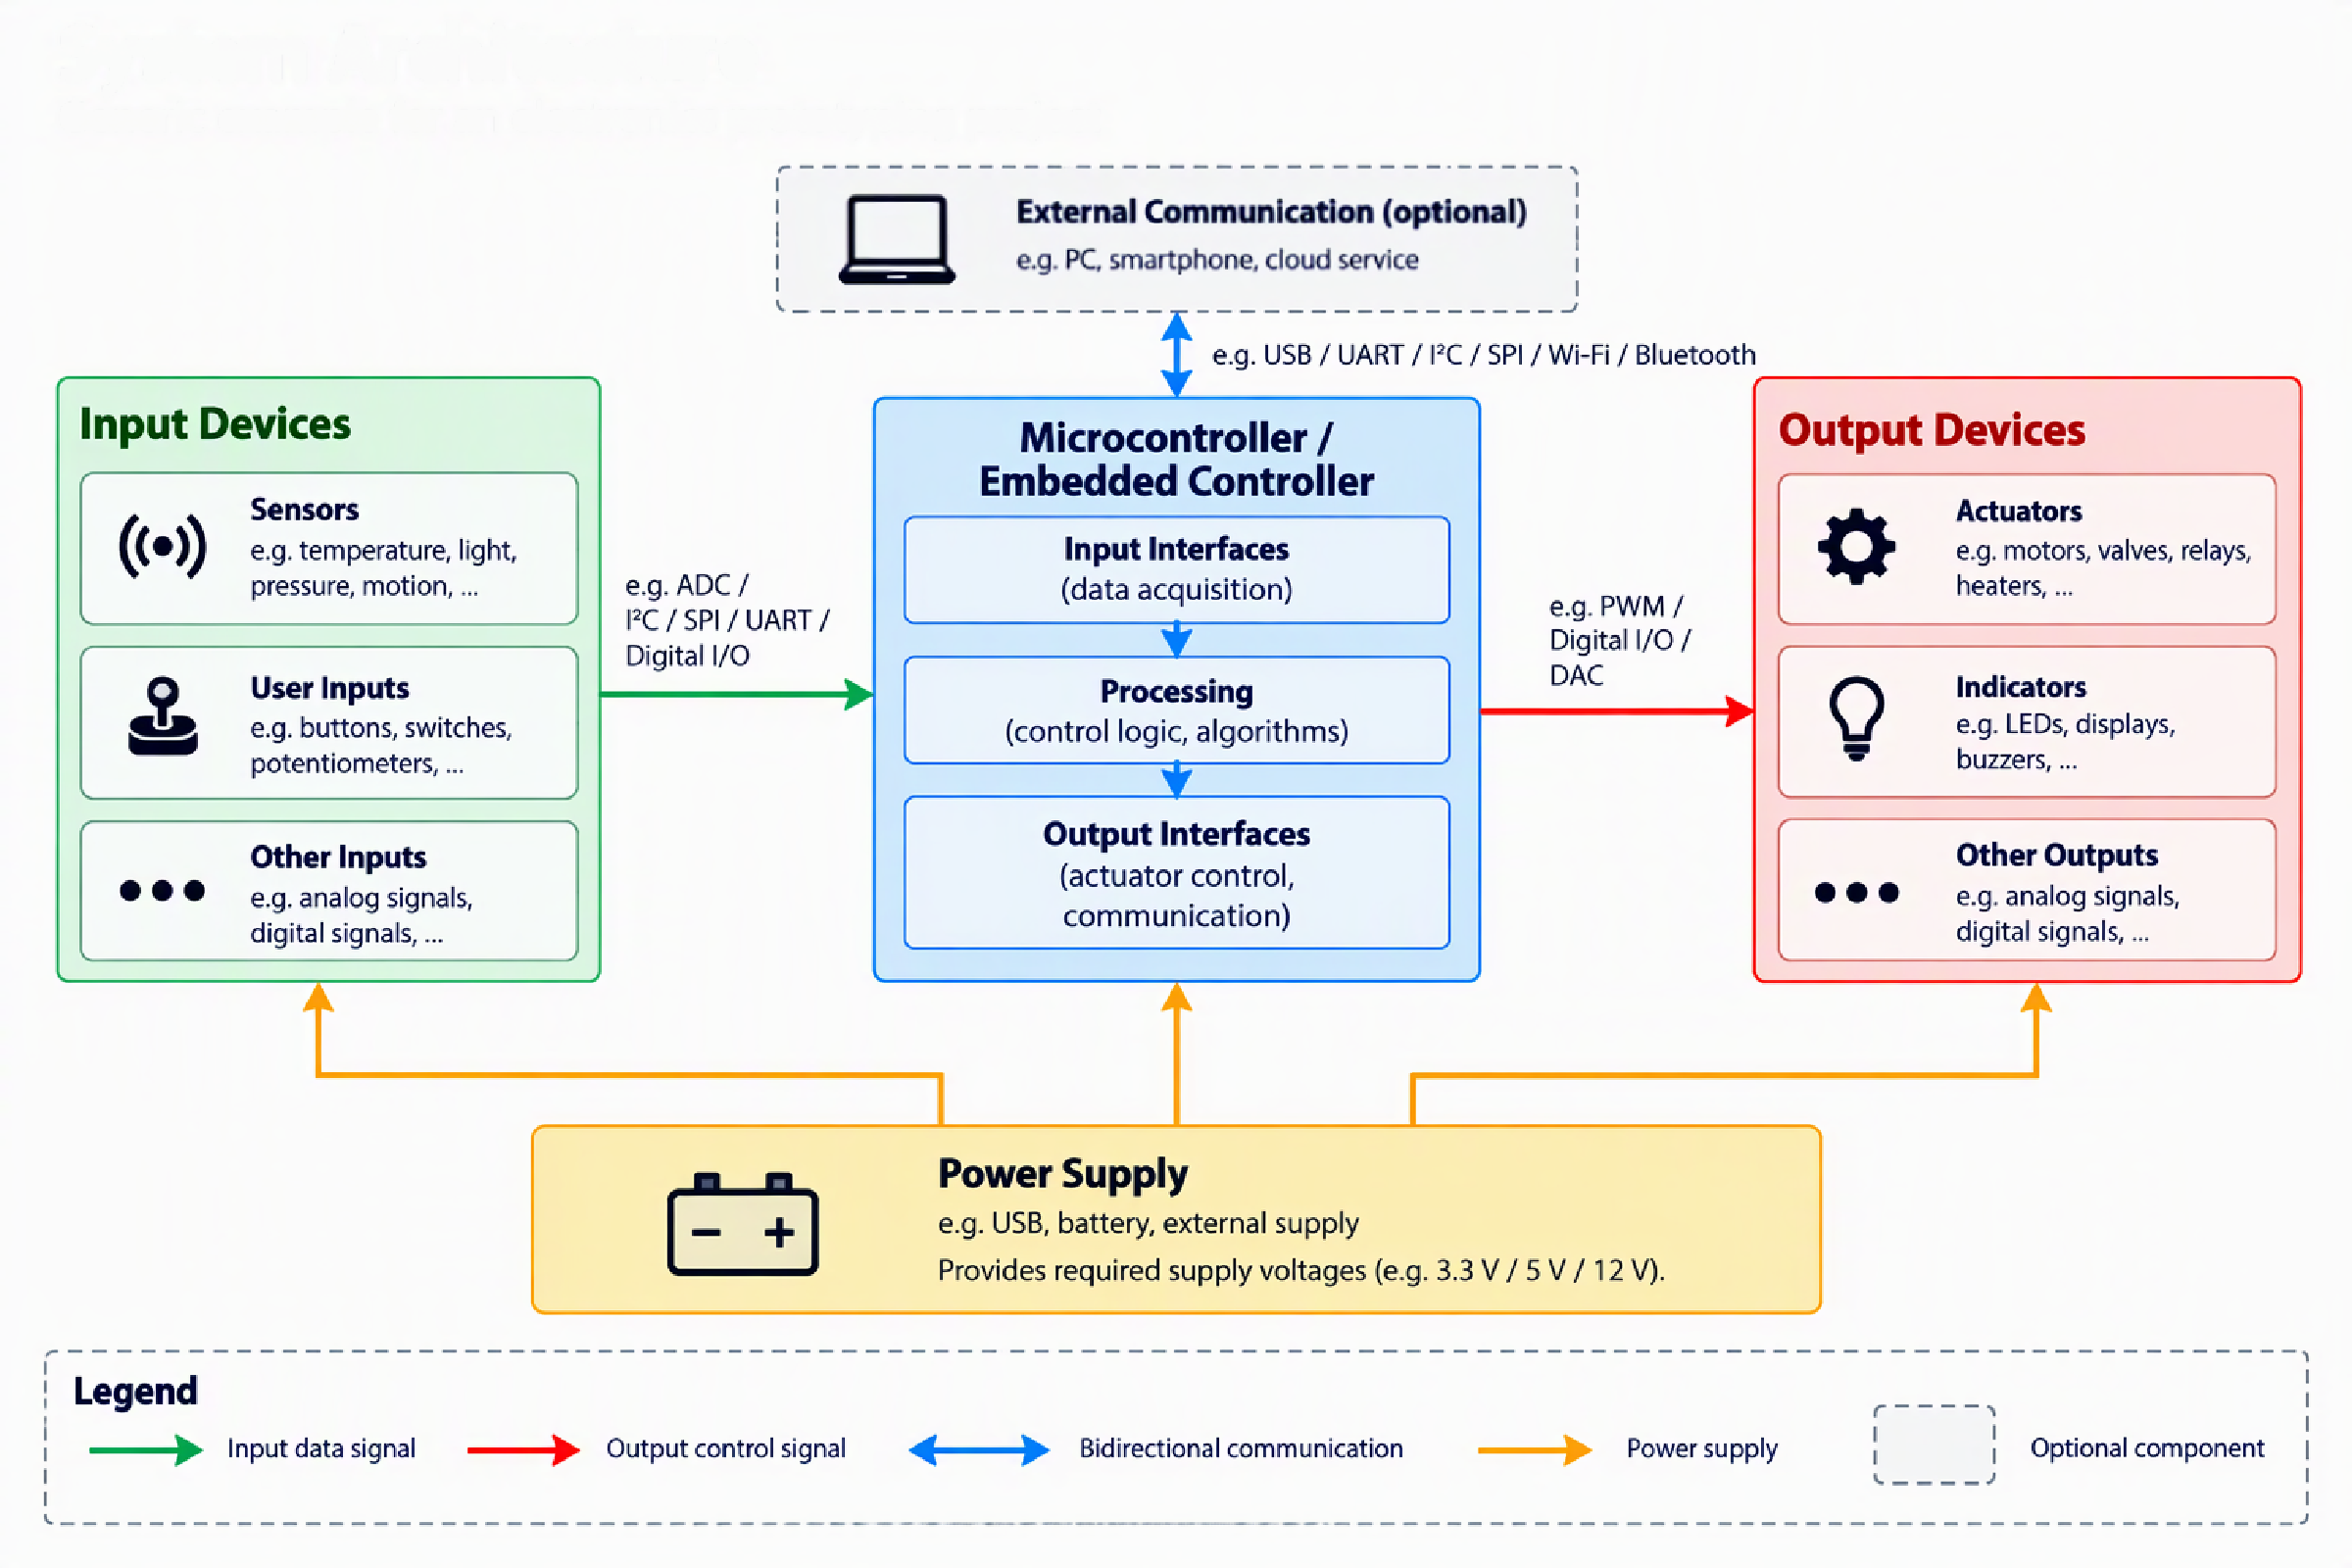
\includegraphics[width=0.9\linewidth]{images/system-architecture.pdf}
  \caption{Example system architecture diagram. Replace with a diagram of 
  the implemented demonstrator, showing the relevant components, interfaces, 
  and direction of data and control flow.}
  \label{fig:architecture}
\end{figure}

% Explain sensor acquisition, signal processing, scaling, and invalid readings.
\section{PSOC acquisition and processing}

Document the PSOC device and any external processing devices, including their
roles and relevant configuration. Describe sensor sampling frequency, signal
conditioning, conversion, filtering or other processing, units and scaling,
timing, and how invalid, missing, or out-of-range readings are handled.
Describe the path from the physical measurement to the displayed or otherwise
used value. Give enough detail to reproduce the configured behavior without
reproducing the entire source code.

% Describe how users operate the demonstrator and receive system feedback.
\section{Interaction and feedback}

Explain how a user operates the demonstrator, what information is presented,
and how the system provides feedback (for example, visual, audible, or
haptic). State how the user can interpret the readings and any status or
error indications. Include photographs of the completed demonstrator showing
its physical construction, sensor placement, and relevant user-interface
elements. Describe relevant interface design decisions and, if a
user-understanding evaluation was conducted, discuss its results in
Chapter~\ref{sec:results}.

% Record implementation details and the calibration method or its absence.
\section{Implementation and calibration}

Summarize the final implementation, including firmware/software versions,
important configuration, assembly, and any dependencies. Describe the
physical construction, mounting arrangements, and relevant mechanical
components. Include CAD models or manufacturing details where necessary to
understand or reproduce the implementation. Describe any calibration or
adjustment procedures performed, including the methods, reference equipment,
and relevant parameters. If no calibration was performed, state this
explicitly and discuss any implications for measurement accuracy.

% Identify relevant hazards, safeguards, limits, and operating precautions.
\section{Safety}

Identify relevant electrical, physical, environmental, and user risks.
Describe implemented safeguards, operating limits, and any precautions
required during setup and testing. Do not imply certification or safety
validation beyond the evidence available.
